\subsection{Definitioner}

\paragraph{Definition av en funktion}

Låt $X, Y$ vara mängder. En funktion $f: X\to Y$ är ett sätt att till varje element $x \in X$ tilldela ett välbestämt element $y\in Y$. Vi säger att $x$ avbildas på $y$ och att $y$ är bilden av $x$. $x$ kallas argumentet till $f$. $X$ kallas funktionens definitionsmängd, och betecknas även $D_f$. $Y$ kallas funktionen målmängd.

\paragraph{Värdemängd}

Värdemängden till $f: X\rightarrow Y$ definieras som:
\begin{align}
	V_f=\left \{y\in Y: y=f(x)\textnormal{ för något }x\in X\right \}\nonumber
\end{align}
alltså alla värden $f$ antar.

\paragraph{Injektivitet}

$f$ är injektiv om det för varje $x_1, x_2 \in X$ gäller att om $f(x_1)=f(x_2)$ så är $x_1=x_2$.

\paragraph{Surjektivitet}

$f$ är surjektiv om $V_f=Y$.

\paragraph{Bijektivitet}

Om $f$ är injektiv och surjektiv, är $f$ bijektiv.

\paragraph{Inversa funktioner}

Låt $f: X \to Y$ vara en bijektiv funktion. Inversen till $f$ är avbildningen $f^{-1}: Y\to X$ som ges av $f^{-1}(y)=x$, där $y=f(x)$. Funktioner som har en invers kallas inverterbara.

\paragraph{Växande och avtagande funktioner}

En funktion $f$ är växande på en mängd $M\in D_f$ om det för varje $x,y\in M: x<y$ gäller att $f(x)\leq f(y)$. Om $M=D_f$ kallas $f$ växande. Avtagande funktioner definieras analogt.

\paragraph{Strängt växande och avtagande funktioner}

En funktion $f$ är strängt växande på en mängd $M\in D_f$ om det för varje $x,y\in M: x<y$ gäller att $f(x)<f(y)$. Om $M=D_f$ kallas $f$ strängt växande. Strängt avtagande funktioner definieras analogt.

\paragraph{Monotona funktioner}

Om en funktioner är antingen strängt växande respektiva strängt avtagande eller växande respektiva avtagande i ett intervall, är den strängt monoton respektiva monoton.

\paragraph{Uppåt och nedåt begränsade funktioner}

En funktion $f$ är uppåt begränsad om $V_f$ är uppåt begränsad. Nedåt begränsade funktioner definieras analogt. Om funktioner saknar övre eller nedra begrensning är den uppåt eller nedåt obegränsad.

\paragraph{Trigonometriska funktioner}

Betrakta enhetssirkeln i figur \ref{fig:unit_circle}, med radie $1$.

\begin{figure}[!ht]
	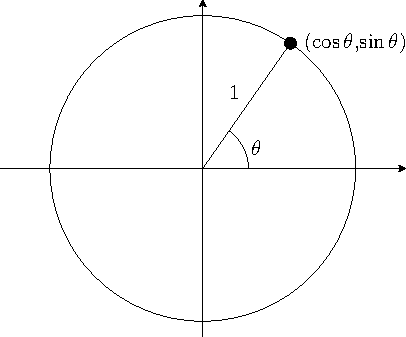
\includegraphics[width=\linewidth]{./Images/unit_circle/unit_circle.pdf}
	\caption{Enhetssirkeln.}
	\label{fig:unit_circle}
\end{figure}

Man tenker sig en punkt på cirkeln enligt figuren, var linjen från cirkelns centrum till cirkeln bildar en vinkel $\theta$ med $x$-axeln. Denna vinkeln startar när punkten på cirkeln ligger på den positiva sidan av $x$-axeln, och ökar moturs. Från denna konstruktionen definieras $\sin$ och $\cos$ utifrån $x$- och $y$-koordinaterna till punkten för en given $\theta$, var $\theta$ mäts i radianer. Vi definierar även $\tan\theta=\frac{\sin\theta}{\cos\theta}$.

Från definitonerna ser vi at $\sin x$ och $\cos x$ är definierade för alla $x\in\mathbb{R}$, medan $\tan x$ är definierad för alla $x\neq \frac{\pi}{2}n, n\in\mathbb{Z}$.

\paragraph{Radianer}

Radianer är ett mått på vinklar som är baserad på enhetscirkeln. Om man tenker sig att punkten i figur \ref{fig:unit_circle} beväger sig från startpunktet och till nån 

\paragraph{Trigonometriska funktioners egenskaper}

Från definitionen av dom trigonometriska funktionerna följer många egenskaper vid dissa. Några essensiella är listad under:

\begin{align*}
	&\cos^2x + \sin^2x = 1\\
	&\sin\left(\theta + 2\pi n\right) = \sin\theta\\
	&\cos\left(\theta + 2\pi n\right) = \cos\theta\\
	&\sin\left(\theta - \frac{\pi}{2}\right) = \cos\theta\\
	&\cos\left(\theta + \frac{\pi}{2}\right) = \sin\theta\\
	&\sin\left(-\theta\right) = -\sin\theta\\
	&\cos\left(-\theta\right) = -\cos\theta\\
	&\sin\left(\theta+\pi\right) = -\sin\theta\\
	&\cos\left(\theta+\pi\right) = -\cos\theta
\end{align*}

\paragraph{Inversa trigonometriska funktioner}

Låt $f:\left[-\frac{\pi}{2},\frac{\pi}{2}\right]\to [-1,1]$ sådan att $f(x)=\sin x$. Inversen till denna funktionen betecknas $f^{-1}(x)=\arcsin x$.

Låt $f:[0,\pi]\to [-1,1]$ sådan att $f(x)=\cos x$. Inversen till denna funktionen betecknas $f^{-1}(x)=\arccos x$.

Låt $f:(-\inf,\inf)\to \left[-\frac{\pi}{2}\right],\frac{\pi}{2}]$ sådan att $f(x)=\tan x$. Inversen till denna funktionen betecknas $f^{-1}(x)=\arctan x$.

\paragraph{Exponentialfunktionen}

I häftet definieras inte exponentialfunktionen $a^x, a>1$, utan den antas vara en strängt växande funktion med värdemängd $(0,\inf)$ som uppfyller
\begin{align*}
	&a^0 = 1\\
	&a^1 = a\\
	&a^{x + y} = a^x a^y\\
	&a^{-x} = \frac{1}{a^x}\\
	&\left(a^x\right)^y = a^{xy}
\end{align*}

\paragraph{Logaritmfunktionen}

Låt $f:\mathbb{R}\to (0,\inf)$ sådan att $f(x) = a^x$ för något $a > 1$. Inversen till denna funktionen betecknas som $f^{-1}(x) = \log_a x$.

\paragraph{Absolutbelopp}

Absolutbeloppet definieras som $\abs{x} = \sqrt{x^2}$. Detta impliserar att
\begin{align*}
	\abs{x} =
	\begin{cases}
		-x, & x < 1\\
		x,  & x \geq 1
	\end{cases}
\end{align*}
 
\subsection{Satser}

\paragraph{Trigonometriska funktioner med vinkelsummor}
\begin{align*}
	\sin\left(x+y\right) = \sin x\cos y + \cos x\sin y\\
	\cos\left(x+y\right) = \cos x\cos y - \sin x\sin y
\end{align*}

\paragraph{Cosinussatsen}

Låt $a,b,c$ vara sidorna i en triangel och $\theta$ vinkeln där sidlängderna $a$ och $b$ möts. Då gäller att
\begin{align*}
	c^2=a^2+b^2-2ab\cos\theta
\end{align*}

\paragraph{Logaritmfunktionens egenskaper}

Låt $a > 1$. Då gäller att
\begin{align}
	&\log_a 1 = 0 \label{eq:log_1}\\
	&\log_a\left(xy\right) = \log_a\left(x\right) + \log_a\left(y\right) \label{eq:log_prod}\\
	&\log_a\left(x^y\right) = y\log_a\left(x\right) \label{eq:log_pow}
\end{align}

\subparagraph{Bevis}

Alla identiteter är baserade på inverterbarheten till exponentialfunktionen - $a^{\log_a x} = x$ - och injektiviteten till exponentialfunktionen, samt reglerna som exponentialfunktionen uppfyllar.

Ekvation \ref{eq:log_1} fås från att $a^{\log_a 1} = 1$ och att $a^0 = 1$. Eftersom exponentialfunktionen är injektiv, är det bevisad.

Ekvation \ref{eq:log_prod} fås från att $a^{\log_a xy} = xy$ och att $a^{\log_a x + \log_a y} = a^{\log_a x}a^{\log_a y}=xy$.

Ekvation \ref{eq:log_pow} fås från att $a^{\log_a x^y} = x^y$ och att $a^{y\log_a x} = \left(a^{\log_a x}\right)^y = x^y$.

\paragraph{Absolutbeloppens egenskaper}

\begin{align}
	&\abs{xy} = \abs{x}\abs{y} \label{eq:abs_prod} \\
	&\abs{x + y} \leq \abs{x} + \abs{y} \label{eq:abs_sum}
\end{align}

\subparagraph{Bevis}

Kommer kanskje någon gång.